\chapter{Картинки}\label{ch:fig}

Рисунки следует готовить в хорошем качестве. Современные графические приложения как правило позволяют создавать графики в \href{https://ru.wikipedia.org/wiki/%D0%92%D0%B5%D0%BA%D1%82%D0%BE%D1%80%D0%BD%D0%B0%D1%8F_%D0%B3%D1%80%D0%B0%D1%84%D0%B8%D0%BA%D0%B0}{векторном} виде и сохранять их в формате \verb|.pdf|, которые затем можно вставлять в \LaTeX\, документы. Если готовите растровые иллюстрации, то старайтесь делать их с высоким \href{https://ru.wikipedia.org/wiki/Dots_per_inch}{DPI} (больше 150, например). Рекомендуется по возможности  использовать форматы без потери качества (например \verb|.png|).

О вставке изображений:

\begin{itemize}
	\item \href{http://mydebianblog.blogspot.com/2008/12/latex_15.html}{http://mydebianblog.blogspot.com/2008/12/latex\_15.html}
	\item \href{http://mydebianblog.blogspot.com/2013/03/amorua-advanced-floats.html}{http://mydebianblog.blogspot.com/2013/03/amorua-advanced-floats.html}
	\item \href{https://www.overleaf.com/learn/latex/Inserting_Images}{https://www.overleaf.com/learn/latex/Inserting\_Images}
	\item \href{https://www.overleaf.com/learn/latex/Positioning_of_Figures}{https://www.overleaf.com/learn/latex/Positioning\_of\_Figures}
\end{itemize}







\begin{figure}[h]
	\centering
	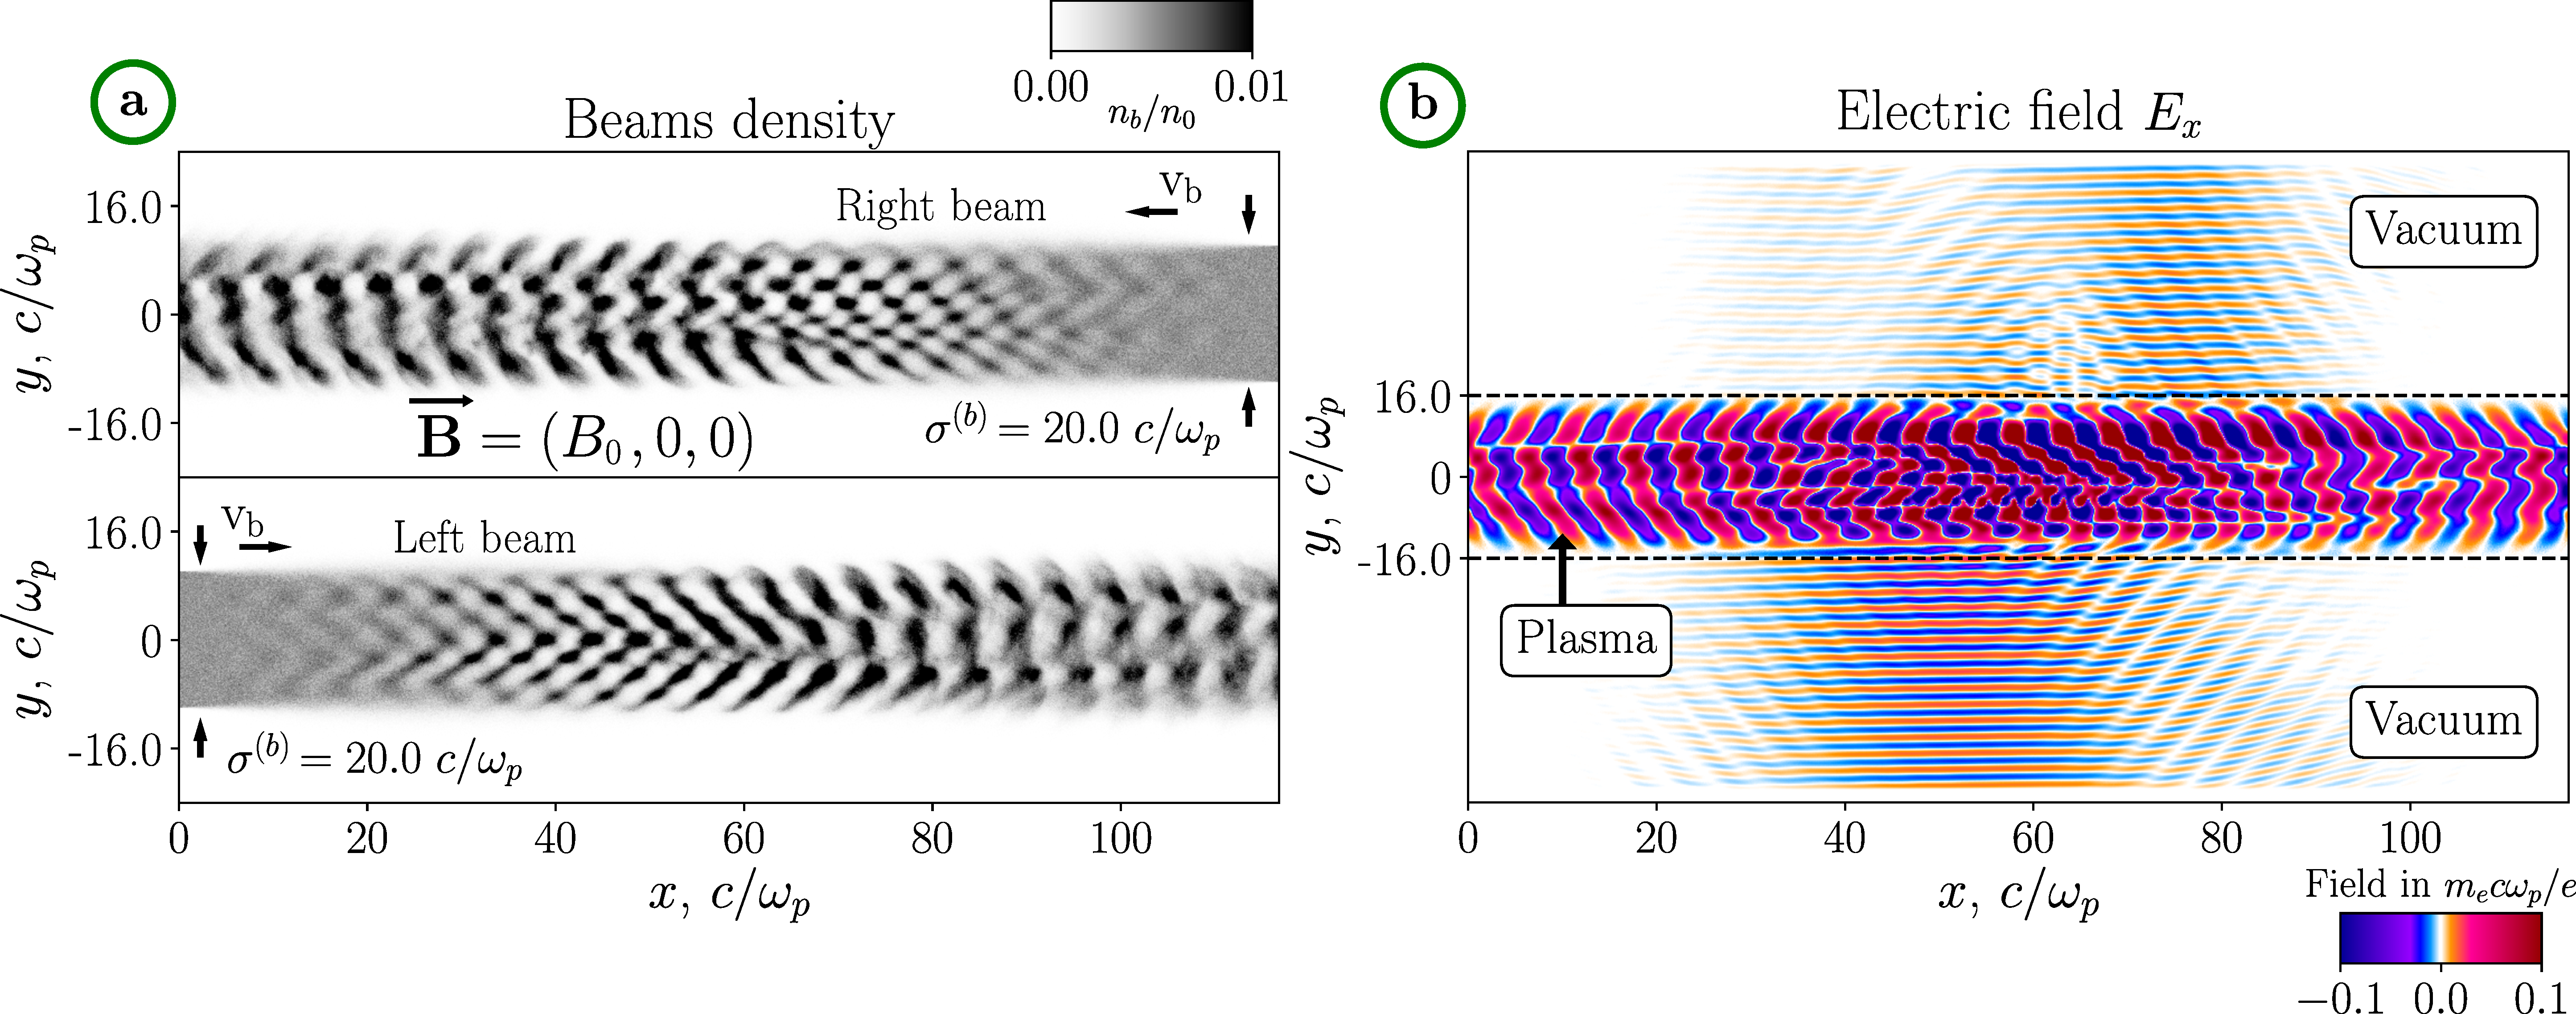
\includegraphics[width=0.95\linewidth]{fig2.pdf}
	\caption{Одна картинка по центру размером 0.95 длины строки}
	\label{fig:image1}%ссылка на картинку
\end{figure}


\begin{figure}[h]
	\begin{center}
		\begin{minipage}[h]{0.45\linewidth}
			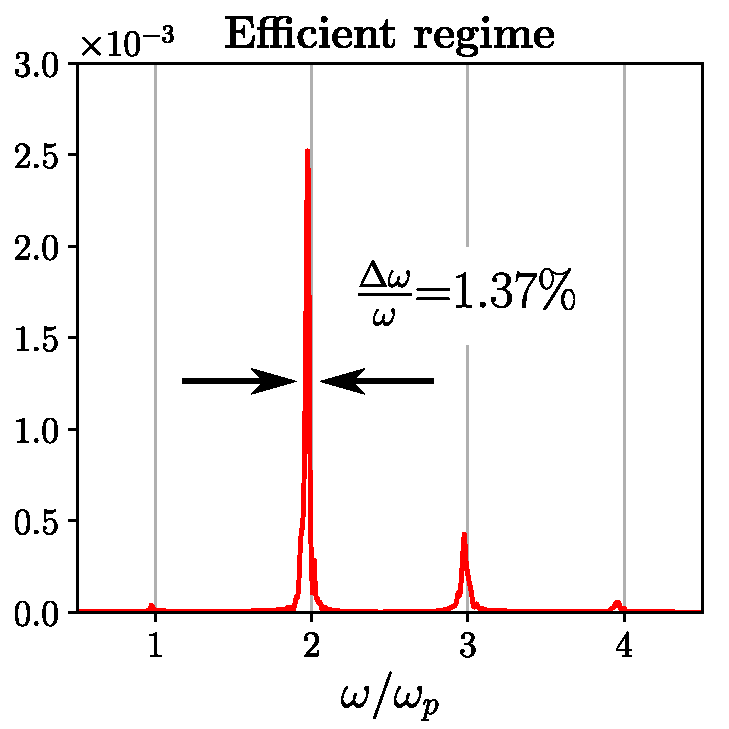
\includegraphics[width=1\linewidth]{fig09}
			\caption{Два изображения в строчку.} %% подпись к рисунку
			\label{fig:image2} %% метка рисунка для ссылки на него
		\end{minipage}
		\hfill
		\begin{minipage}[h]{0.45\linewidth}
			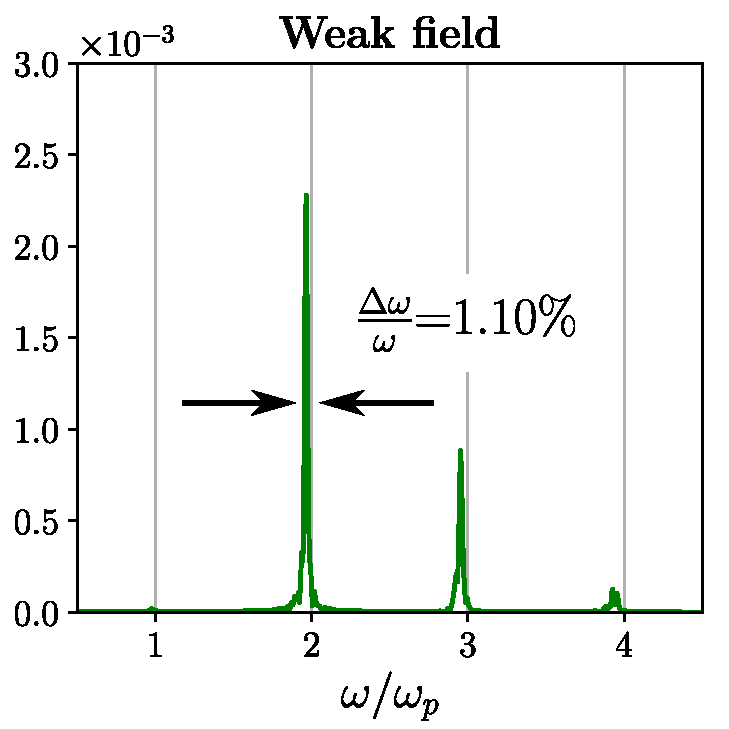
\includegraphics[width=1\linewidth]{fig10}
			\caption{С индивидуальными подписями.}
			\label{fig:image3}
		\end{minipage}
	\end{center}
\end{figure}


\section{С обтеканием}
\lipsum[1-2]

\begin{wrapfigure}[12]{r}{0.45\linewidth} 

	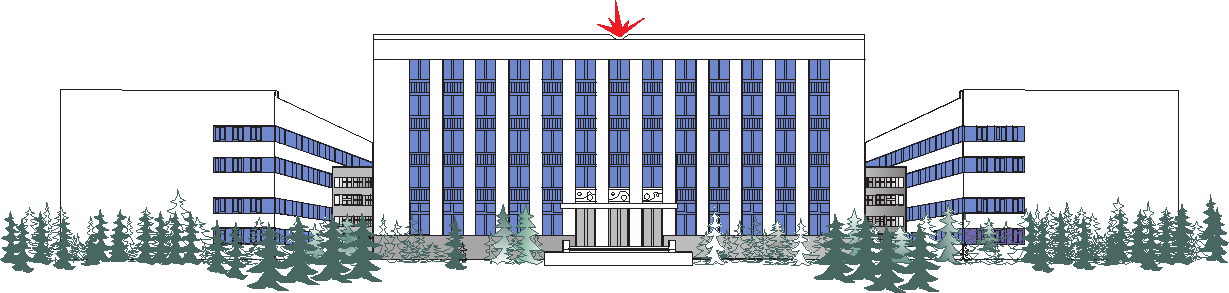
\includegraphics[width=\linewidth]{binpW.pdf}
	\caption{Рисунок с обтеканием. [12] - определяет высоту рисунка в число строк текста и позволяет отбить дополнительное место для рисунков. {r} - положение картинки на странице, можно слева {l} или справа {r}. 
	}
	\label{fig:image4}
\end{wrapfigure}


\lipsum[1-2]

Для рисунков с обтеканием необходим пакет

\verb|\usepackage{wrapfig}%картинки с обтеканием| 

Но вообще картинки с обтеканием лучше не делать.

\section{Изображения с подписями в \LaTeX}

Современные приложения позволяют создавать изображения с текстом, сразу пропущенным через \LaTeX. 

\subsection{matplotlib}
Например в \verb|python| достаточно использовать в модуле \verb|matplotlib| следующую преамбулу:


\begin{minted}{python}
   rc('text', usetex=True)
   rc('font', family='serif')
   rc('text.latex', 
   preamble=r"\usepackage[english,russian]{babel}")
\end{minted}

Это позволит использовать в подписях текст на русском языке, написанный шрифтом с засечками. Также в \verb|matplotlib| можно писать формулы по правилам \LaTeX'а: \verb*|$2+5=7$|
Подробнее:
\begin{itemize}
	\item \href{https://matplotlib.org/stable/tutorials/text/usetex.html?highlight=latex}{https://matplotlib.org/stable/tutorials/text/usetex.html?highlight=latex}
	\item \href{https://pyprog.pro/mpl/mpl_latex_title.html}{https://pyprog.pro/mpl/mpl\_latex\_title.html}
	\item \href{http://s.arboreus.com/2009/04/cyrillic-letters-in-matplotlibpylab.html}{http://s.arboreus.com/2009/04/cyrillic-letters-in-matplotlibpylab.html}
\end{itemize}

\subsection{gnuplot}

Также это можно делать в \verb*|gnuplot|'е: 

\href{http://www.gnuplot.info/docs/tutorial.pdf}{http://www.gnuplot.info/docs/tutorial.pdf}

В самом \LaTeX'е есть возможность строить графики \verb*|gnuplot|'ом с помощью пакета \href{https://mirror.truenetwork.ru/CTAN/macros/latex/contrib/gnuplottex/gnuplottex.pdf}{gnuplottex}.

 Пример использования:  \href{https://habr.com/ru/post/250087/}{https://habr.com/ru/post/250087/}


